\chapter{beatific bursts} 
\label{sec:bursts}
\rhead[]{\leftmark}
\lstset{style=6502Style}
\lstset{ 
   aboveskip=5pt,
   belowskip=0pt,
}

\begin{definition}[Jeffrey Says\index{Jeffrey Says}]
\setlength{\intextsep}{0pt}%
\setlength{\columnsep}{3pt}%
\begin{wrapfigure}{l}{0.12\textwidth}

\includegraphics[width=\linewidth]{src/callout/psych.png} 
\end{wrapfigure}
\small
These allow you to preprogram and recall at will
instantaneous flashes on the screen. Set up symmetry and
smoothing delay as required, then press SHIFT plus the fkey to
which you want to assign your FX. Move the cursor to where you
want a burst then press Left-Arrow to enter that point. Do this up to
16 times. Press RETURN when done. Pressing the fkey thus
assigned stuffs all the points you defined into the buffer
instantaneously. Don’t worry about it - try the ones I've defined!
\end{definition}

Bursts are short pre-programmed sequences of patterns that can be invoked using the Function keys.
This allows the player to define up to four different burst sequences, one per function key. A burst
can consist of up to 16 different patterns displayed in 16 different positions on the screen. Each burst
has a defined symmetry and smoothing delay. The greater the smoothing delay, the longer the pattern
will stay on screen.

The bursts are programmable, the player can define new ones through the slightly finicky process of pressing
Shift and the corresponding Function key, then selecting the different points on the screen for each of up
to 16 patterns to appear. You can see the data structure that supports this on the following page. Note
that the symmetry and smoothing delay are set for the burst sequence as a whole, but each element of the
burst sequence has its own pattern and position co-ordinates.

\clearpage
\begin{figure}[H]
    \centering
    \begin{adjustbox}{width=12cm,center}
      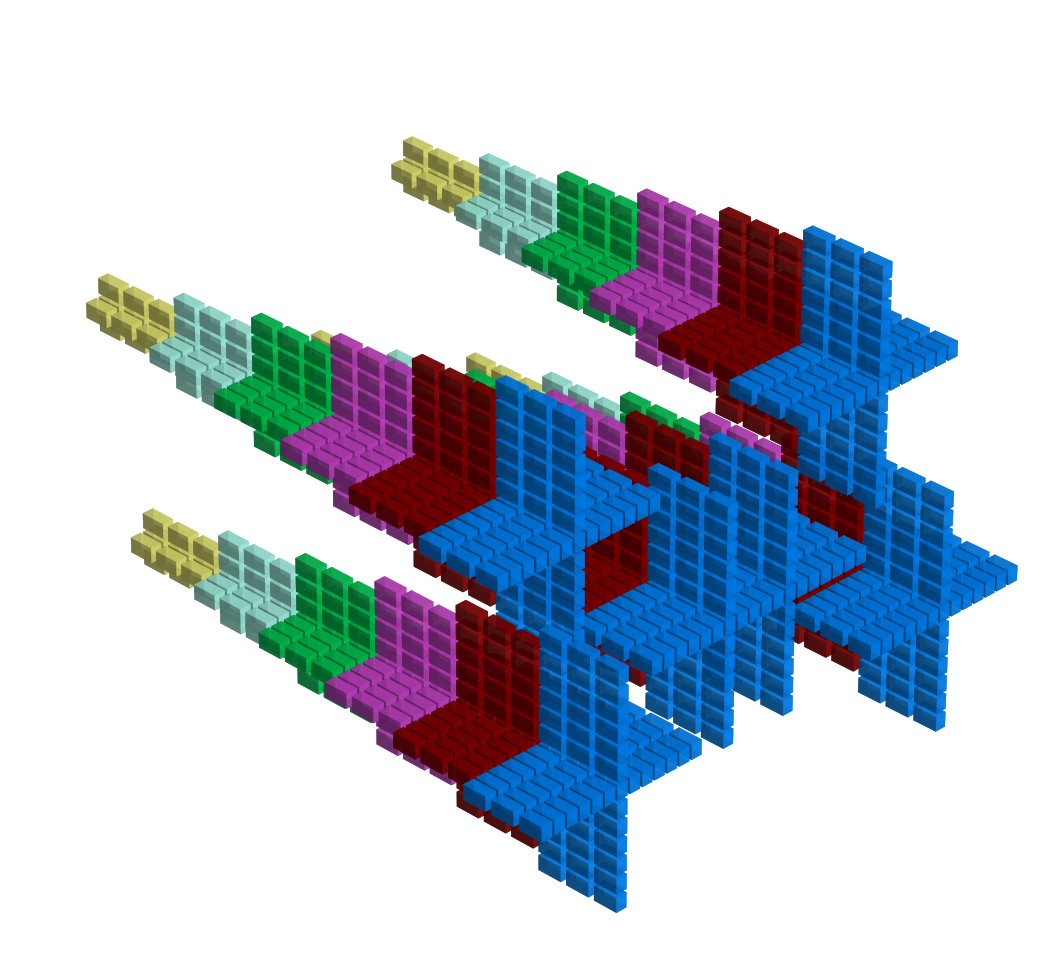
\includegraphics[width=12cm]{src/patterns/bursts/pattern0-45.png}%
    \end{adjustbox}
\caption{Evolution of the default burst at F1.}
\end{figure}
\clearpage

\rhead[]{F1 Burst}
\begin{lstlisting}[caption=Source code for the F1 Burst.,escapechar=\%]
burstGeneratorF1%\index{burstGeneratorF1}% = $C200
  ; currentSymmetrySetting%\index{currentSymmetrySetting}%: 'Current symmetry setting.'
  ; Possible values are 0 - 4:
  ; 'NO SYMMETRY     '
  ; 'Y-AXIS SYMMETRY '
  ; 'X-Y SYMMETRY    '
  ; 'X-AXIS SYMMETRY '
  ; 'QUAD SYMMETRY   '
  .BYTE $01
  ; smoothingDelay%\index{smoothingDelay}%: 'Because of the time taken to draw larger patterns
  ; speed increase-decrease is not linear. You can adjust the 
  ; compensating delay which often smooths out jerky patterns. 
  ; Can be used just for special FX) though. Suck it and see.'
  .BYTE $0C

  ; Burst Position 1
  ; X/Y Co-ordinates: X/Y Position relative to cursor to place the
  ; burst.
  .BYTE $07,$06
  ; Index to pattern in patternIndexArray%\index{patternIndexArray}%
  .BYTE PULSAR

  ; Burst Position 2
  ; X/Y Co-ordinates: X/Y Position relative to cursor to place the
  ; burst.
  .BYTE $11,$0D
  ; Index to pattern in patternIndexArray%\index{patternIndexArray}%
  .BYTE PULSAR

  ; Burst Position 3
  ; X/Y Co-ordinates: X/Y Position relative to cursor to place the 
  ; burst.
  .BYTE $06,$11
  ; Index to pattern in patternIndexArray%\index{patternIndexArray}%
  .BYTE PULSAR

  ; - An $FF in the first byte of 'X/y Co-ordinates' indicates the
  ; end of the data, e.g. in 'Burst Position 4' below.
  ; Burst Position 4
  ; X/Y Co-ordinates: X/Y Position relative to cursor to place the 
  ; burst.
  .BYTE $FF,$0B
  ; Index to pattern in patternIndexArray%\index{patternIndexArray}%
  .BYTE PULSAR

\end{lstlisting}

\clearpage
\textbf{Lines 1189-1231. \icode{\textbf{CheckKeyboardInput\index{CheckKeyboardInput}}}}
\begin{lstlisting}[escapechar=\%]
functionKeys .BYTE $04,$05,$06,$03
;-------------------------------------------------------
; CheckKeyboardInput%\index{CheckKeyboardInput}%
;-------------------------------------------------------
CheckKeyboardInput%\index{CheckKeyboardInput}%   
        ...
CheckForKeyStroke   
        LDA lastKeyPressed%\index{lastKeyPressed}%
        ...

MaybeFunctionKeysPressed   
        ; Was one of the function keys pressed?
        LDX #$00
FnKeyLoop   
        CMP functionKeys,X
        BEQ FunctionKeyWasPressed ; One of them was pressed!
        INX 
        CPX #$04
        BNE FnKeyLoop

        ; Continue checking
        JMP MaybeQPressed%\index{MaybeQPressed}%

        ; A Function key was pressed, ignore if the 
        ; sequencer is active.
FunctionKeyWasPressed   
        STX functionKeyIndex%\index{functionKeyIndex}%

        LDA sequencerActive%\index{sequencerActive}%
        BNE MaybeQPressed%\index{MaybeQPressed}%

        LDA #SEQUENCER_ACTIVE
        STA currentVariableMode%\index{currentVariableMode}%
        JSR LoadOrProgramBurstGenerator%\index{LoadOrProgramBurstGenerator}%
        RTS 

        ...
\end{lstlisting}
\clearpage

\rhead[]{\icode{CheckKeyboardInput\index{CheckKeyboardInput}}}
\begin{wrapfigure}{r}{0.15\textwidth}
\frame{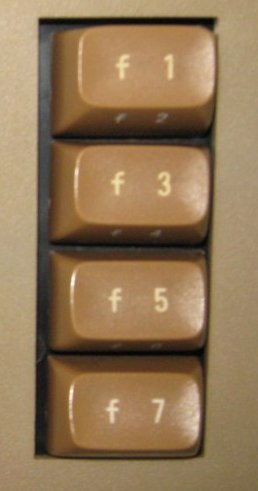
\includegraphics[width=2cm]{src/bursts/fn_keys_only.jpg}}%
\end{wrapfigure}
\textbf{Lines 1189-1231. \icode{\textbf{CheckKeyboardInput\index{CheckKeyboardInput}}}:} This is the routine that detects when the player has selected a new
Burst by pressing one of the four 'Function' keys (picured to the right). It is part of the much larger routine \icode{CheckKeyboardInput\index{CheckKeyboardInput}} which periodically checks
for keyboard input by polling the byte at address \icode{\$00C5} (which we label \icode{lastKeyPressed\index{lastKeyPressed}}). This address always
contains the value of the most recently pressed key on the keyboard.

\textbf{Lines 1189-1231. \icode{\textbf{MaybeFunctionKeysPressed}}:} The ellipses before this statement indicated all the code we've
left out in the listing opposite. As you might guess, the absent code is checking for lots of other keys you are likely to have pressed but
this function checks whether you pressed one of the 4 Function keys we're interested in. Note that it's a loop, checking for each of the 4
function key values stored in \icode{functionKeys}. If we actually hit one, the loop breaks and calls \icode{FunctionKeyWasPressed}. Otherwise
it reaches \icode{JMP MaybeQPressed\index{MaybeQPressed}} and calls that function instead - in other words continues on checking for other keys you might have
pressed.

\textbf{Lines 1189-1231. \icode{\textbf{FunctionKeyWasPressed}}:} So if we get here a Function key was pressed! Since we broke out of \icode{FnKeyLoop}
when we hit one, the actual function key that we hit is stored in the \icode{X} register. So first we save that off in a bit of storage called
\icode{functionKeyIndex\index{functionKeyIndex}} for use later. Since the Sequencer (which we will come to in the next chapter) shares functionality with the Burst generator
we don't let them both be active at the same time. If the Sequence is not currently active we're free to do some bursting. We set our little state
variable called \icode{currentVariableMode\index{currentVariableMode}} which keeps track of any fancy business we're doing with the information that we're about to do some 
burst activation and call the routine that will actually load a burst for us: \icode{LoadOrProgramBurstGenerator\index{LoadOrProgramBurstGenerator}}.


\clearpage
\begin{figure}[H]
    \centering
    \begin{adjustbox}{width=12cm,center}
      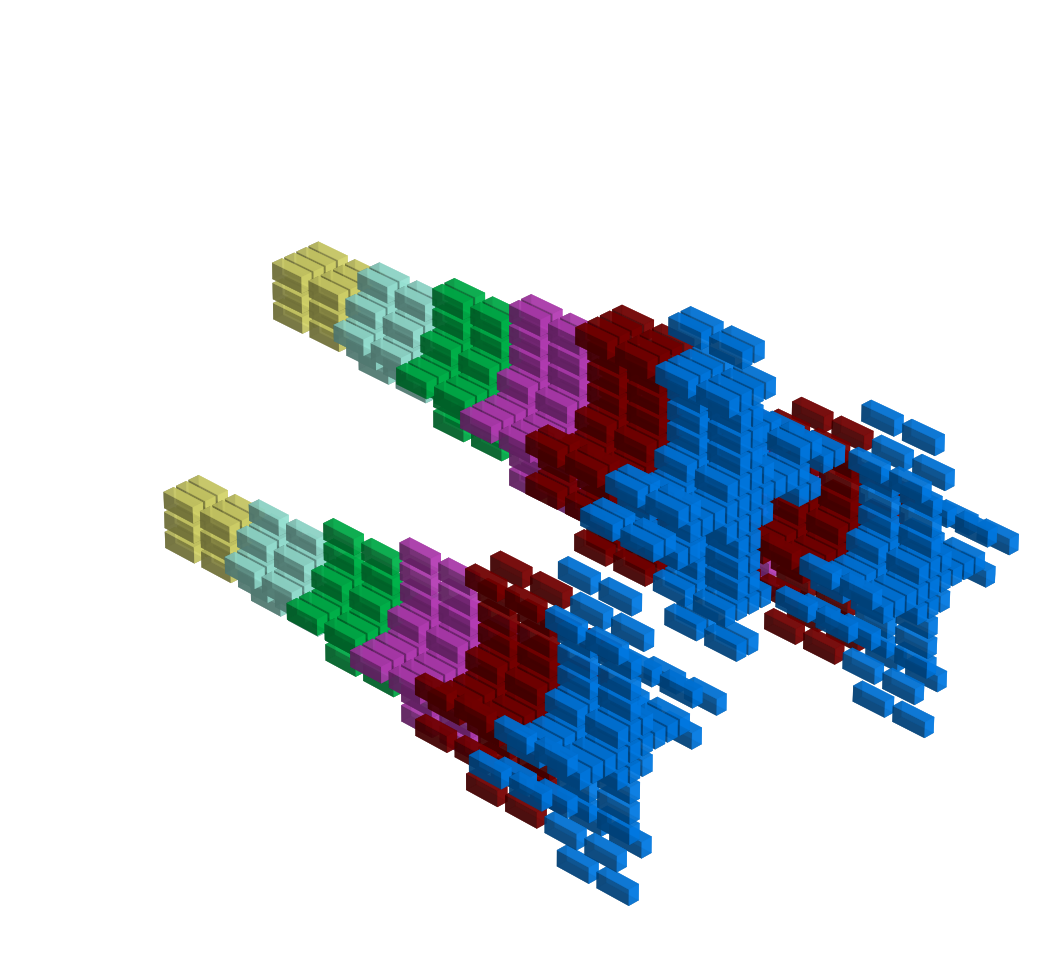
\includegraphics[width=12cm]{src/patterns/bursts/pattern1-45.png}%
    \end{adjustbox}
\caption{Evolution of the default burst at F3.}
\end{figure}
\clearpage

\rhead[]{F3 Burst}
\begin{lstlisting}[caption=Source code for the F3 Burst.,escapechar=\%]
burstGeneratorF3%\index{burstGeneratorF3}% = $C220
  ; currentSymmetrySetting%\index{currentSymmetrySetting}%: 'Current symmetry setting.'
  ; Possible values are 0 - 4:
  ; 'NO SYMMETRY     '
  ; 'Y-AXIS SYMMETRY '
  ; 'X-Y SYMMETRY    '
  ; 'X-AXIS SYMMETRY '
  ; 'QUAD SYMMETRY   '
  .BYTE Y_AXIS_SYMMETRY

  ; smoothingDelay%\index{smoothingDelay}%: 'Because of the time taken to draw larger patterns
  ; speed increase/decrease is not linear. You can adjust the 
  ; compensating delay which often smooths out jerky patterns.
  ; Can be used just for special FX) though. Suck it and see.'
  .BYTE $0C

  ; Burst Position 1
  ; X/Y Co-ordinates: X/Y Position relative to cursor to place burst.
  .BYTE $13,$08
  ; Index to pattern in patternIndexArray%\index{patternIndexArray}%
  .BYTE STARONE

  ; Burst Position 2
  ; X/Y Co-ordinates: X/Y Position relative to cursor to place burst.
  .BYTE $07,$0F
  ; Index to pattern in patternIndexArray%\index{patternIndexArray}%
  .BYTE STARONE

  ; Burst Position 3
  ; X/Y Co-ordinates: X/Y Position relative to cursor to place burst.
  .BYTE $FF,$00
  ; Index to pattern in patternIndexArray%\index{patternIndexArray}%
  .BYTE MULTICROSS

\end{lstlisting}

\clearpage
\textbf{Lines 1189-1231. \icode{\textbf{LoadOrProgramBurstGenerator\index{LoadOrProgramBurstGenerator}}}}
\begin{lstlisting}[basicstyle=\ttfamily\scriptsize,escapechar=\%]
functionKeyToSequenceArray
       .BYTE <burstGeneratorF1%\index{burstGeneratorF1}%,<burstGeneratorF3%\index{burstGeneratorF3}%
       .BYTE <burstGeneratorF5,<burstGeneratorF7

;-------------------------------------------------------
; LoadOrProgramBurstGenerator%\index{LoadOrProgramBurstGenerator}%
;-------------------------------------------------------
LoadOrProgramBurstGenerator%\index{LoadOrProgramBurstGenerator}%   
        JSR ClearLastLineOfScreen%\index{ClearLastLineOfScreen}%

        LDA shiftPressed%\index{shiftPressed}%
        AND #$01
        BEQ PointToBurstDataForFunctionKey

        ; Display the data free message
        LDX #$00
DisplayDataFreeLoop   
        LDA txtDataFree,X
        STA lastLineBufferPtr,X
        INX 
        CPX #$10
        BNE DisplayDataFreeLoop
        JSR WriteLastLineBufferToScreen%\index{WriteLastLineBufferToScreen}%

PointToBurstDataForFunctionKey   
        LDA #>burstGeneratorF1%\index{burstGeneratorF1}%
        STA currentSequencePtrHi%\index{currentSequencePtrHi}%
        LDX functionKeyIndex%\index{functionKeyIndex}%
        LDA functionKeyToSequenceArray,X
        STA currentSequencePtrLo%\index{currentSequencePtrLo}%

        LDA shiftPressed%\index{shiftPressed}%
        AND #$01
        BEQ LoadBurstDataInstead

ProgramBurstData
        ; Set the current data free to 16
        LDA #$10
        STA currentDataFree%\index{currentDataFree}%

        ; Store the current symmetry setting and smoothing delay
        ; in the storage selected by the function key. 
        LDY #$00
        LDA currentSymmetrySetting%\index{currentSymmetrySetting}%
        STA (currentSequencePtrLo%\index{currentSequencePtrLo}%),Y
        LDA smoothingDelay%\index{smoothingDelay}%
        INY 
        STA (currentSequencePtrLo%\index{currentSequencePtrLo}%),Y
        RTS 

LoadBurstDataInstead
        LDA #$FF
        STA sequencerActive%\index{sequencerActive}%
        JMP LoadBurstData%\index{LoadBurstData}%

\end{lstlisting}
\clearpage

\rhead[]{\icode{LoadOrProgramBurstGenerator\index{LoadOrProgramBurstGenerator}}}
\textbf{Lines 1189-1231. \icode{\textbf{LoadOrProgramBurstGenerator\index{LoadOrProgramBurstGenerator}}}:} OK, we're either loading a burst of programming one: which is it?
The way we decide this is by finding out if the Shift key was pressed (\icode{LDA shiftPressed\index{shiftPressed}}).. If it was not, then the user wants to load the burst associated with
that Function key and we can skip to \icode{PointToBurstDataForFunctionKey}.

\textbf{Lines 1189-1231. \icode{\textbf{PointToBurstDataForFunctionKey}}:} This is where we make use of a couple of clever steps of preparation
done elsewhere. First of all, the burst data we have (viewable on the pages opposite our pretty pictures) is stored at a number of named locations
which we store in an array called \icode{functionKeyToSequenceArray}:
\begin{lstlisting}[escapechar=\%]
functionKeyToSequenceArray
       .BYTE <burstGeneratorF1%\index{burstGeneratorF1}%,<burstGeneratorF3%\index{burstGeneratorF3}%
       .BYTE <burstGeneratorF5,<burstGeneratorF7
\end{lstlisting}
This means that we can use the \icode{functionKeyIndex\index{functionKeyIndex}} as an index into this array to get the relevant entry for the key that was pressed. 

So for example if F3 was pressed our \icode{functionKeyIndex\index{functionKeyIndex}} has the value \icode{01} and we will here retrieve the value \icode{<burstGeneratorF3\index{burstGeneratorF3}}. This
translates to \icode{\$40}, the low byte of \icode{burstGeneratorF3\index{burstGeneratorF3}}'s location in memory. The high byte is the same for all four of the burst generator
data structures: \icode{\$C2}. This is because they are all located beside each other in memory.

 So we get the high byte from \icode{>burstGeneratorF1\index{burstGeneratorF1}} (\icode{\$C2})
and store it in \icode{currentSequencePtrHi\index{currentSequencePtrHi}} and store our low byte (\icode{\$40}) in \icode{currentSequencePtrLo\index{currentSequencePtrLo}}: we now have a pointer to the data for the burst generator
associated with F3 and are ready to load it. We'll see how this is done on the next page. 

For now though, we check again whether the Shift key is pressed (it isn't) and jump to \icode{LoadBurstDataInstead} and then \icode{LoadBurstData\index{LoadBurstData}} so that we
can get on with, you guessed it, loading the burst data.

\clearpage

\clearpage
\begin{figure}[H]
    \centering
    \begin{adjustbox}{width=12cm,center}
      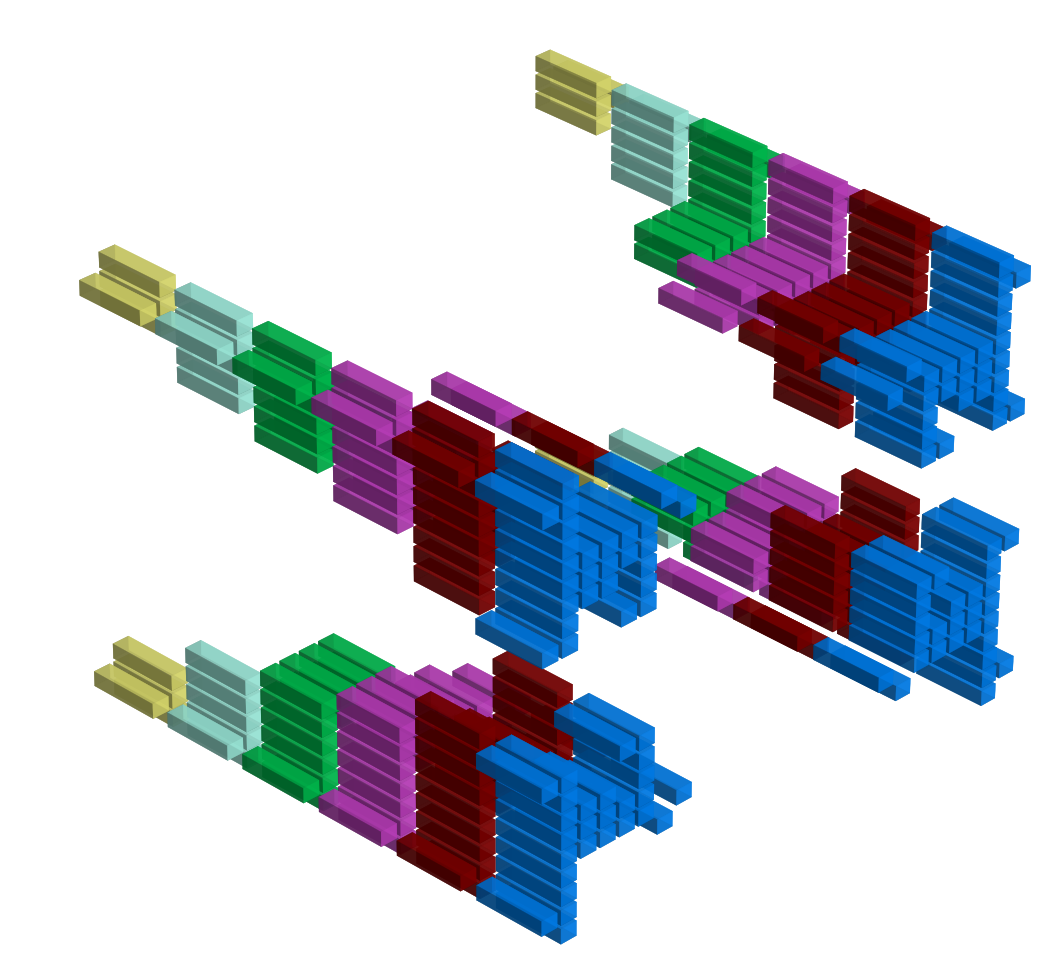
\includegraphics[width=12cm]{src/patterns/bursts/pattern2-45.png}%
    \end{adjustbox}
\caption{Evolution of the default burst at F5.}
\end{figure}
\clearpage

\rhead[]{F5 Burst}
\begin{lstlisting}[caption=Source code for the F5 Burst.,escapechar=\%]
burstGeneratorF5 = $C240
  ; currentSymmetrySetting%\index{currentSymmetrySetting}%: 'Current symmetry setting.'
  ; Possible values are 0 - 4:
  ; 'NO SYMMETRY     '
  ; 'Y-AXIS SYMMETRY '
  ; 'X-Y SYMMETRY    '
  ; 'X-AXIS SYMMETRY '
  ; 'QUAD SYMMETRY   '
  .BYTE QUAD_SYMMETRY
  ; smoothingDelay%\index{smoothingDelay}%: 'Because of the time taken to draw larger patterns
  ; speed increase-decrease is not linear. You can adjust the 
  ; compensating delay which often smooths out jerky patterns. 
  ; Can be used just for special FX) though. Suck it and see.'
  .BYTE $01

  ; Burst Position 1  
  ; X/Y Co-ordinates: X/Y Position relative to cursor to place the burst.
  .BYTE $08,$01
  ; Index to pattern in patternIndexArray%\index{patternIndexArray}%
  .BYTE LALLAMITA

  ; Burst Position 2
  ; X/Y Co-ordinates: X/Y Position relative to cursor to place the burst.
  .BYTE $FF,$01
  ; Index to pattern in patternIndexArray%\index{patternIndexArray}%
  .BYTE LALLAMITA

\end{lstlisting}

\clearpage
\textbf{Lines 1189-1231. \icode{\textbf{LoadBurstData\index{LoadBurstData}}}}
\begin{lstlisting}[escapechar=\%]
;-------------------------------------------------------
; LoadBurstData%\index{LoadBurstData}%
;-------------------------------------------------------
LoadBurstData%\index{LoadBurstData}%    
        LDA #$00
        STA currentVariableMode%\index{currentVariableMode}%

        TAY 
        LDA (currentSequencePtrLo%\index{currentSequencePtrLo}%),Y
        STA symmetrySettingForBurst

        INY 
        LDA (currentSequencePtrLo%\index{currentSequencePtrLo}%),Y
        STA burstSmoothingDelay%\index{burstSmoothingDelay}%

LoadNextBurstPosition    
        LDY #$02
        INC currentStepCount%\index{currentStepCount}%
        LDA currentStepCount%\index{currentStepCount}%
        CMP bufferLength%\index{bufferLength}%
        BNE DontResetStepCountToZero

        ; If currentStepCount%\index{currentStepCount}% would exceed the length of
        ; the arrays, reset it to zero.
        LDA #$00
        STA currentStepCount%\index{currentStepCount}%

DontResetStepCountToZero
        LDX currentStepCount%\index{currentStepCount}%
        LDA currentColorIndexArray%\index{currentColorIndexArray}%,X
        CMP #$FF
        BEQ LoadBurstToBuffers

        LDA shouldDrawCursor
        AND trackingActivated%\index{trackingActivated}%
        BEQ MoveToNextBurstPosition%\index{MoveToNextBurstPosition}%

        STA currentStepCount%\index{currentStepCount}%

        TAX 
        LDA currentColorIndexArray%\index{currentColorIndexArray}%,X

        CMP #$FF
        BNE MoveToNextBurstPosition%\index{MoveToNextBurstPosition}%

\end{lstlisting}
\clearpage

\rhead[]{\icode{LoadBurstData\index{LoadBurstData}}}
\textbf{Lines 1189-1231. \icode{\textbf{LoadBurstData\index{LoadBurstData}}}:} OK we're loading burst data this time, honest.

To load the data we have to know where it is, and we established this in the previous section. The player
pressed F3 so we stored \icode{\$C2} in \icode{currentSequencePtrHi\index{currentSequencePtrHi}} and \icode{\$40} in \icode{currentSequencePtrLo\index{currentSequencePtrLo}}
to represent the address \icode{\$C240} in memory where the burst data for F3 is stored (see the figure on the previous
page also!).

This being the case we can now load the burst data from this address in memory one byte at a time. Let's take as an example the
very first byte we load, which we store in the variable \icode{symmetrySettingForBurst}:
\begin{lstlisting}[escapechar=\%]
        LDA (currentSequencePtrLo%\index{currentSequencePtrLo}%),Y
        STA symmetrySettingForBurst
\end{lstlisting}

With \icode{Y} as zero, this will take the first byte at address \icode{\$C240} and store it. To load the next byte we increment \icode{Y}
and store the second byte (from address \icode{\$C241}) in \icode{burstSmoothingDelay\index{burstSmoothingDelay}}:
\begin{lstlisting}[escapechar=\%]
        INY 
        LDA (currentSequencePtrLo%\index{currentSequencePtrLo}%),Y
        STA burstSmoothingDelay%\index{burstSmoothingDelay}%
\end{lstlisting}

Hopefully you get the idea! Loading the rest of the data for the burst follows the same pattern, but has to deal with the complexity that
while the two settings we just loaded apply to the visualization as a whole, the remaining burst settings come in groups: each group defines
a pattern to draw and a position to draw it at.

\textbf{Lines 1189-1231. \icode{\textbf{LoadNextBurstPosition}}:} This section, which flows on to the following page and forms a loop with the
statement \icode{JMP LoadNextBurstPosition} near the end, is the part that manages loading each group of Burst Positions. 

What it has to do is read in the following data as a group and store it in the right place in our \icode{pixelXPositionArray\index{pixelXPositionArray}/\-pixelYPositionArray\index{pixelYPositionArray}/\-patternIndexArray\index{patternIndexArray}}.
\begin{lstlisting}[escapechar=\%]
  ; Burst Position 1
  ; X/Y Co-ordinates: X/Y Position relative to cursor to place burst.
  .BYTE $13,$08
  ; Index to pattern in patternIndexArray%\index{patternIndexArray}%
  .BYTE STARONE
\end{lstlisting}
As you hopefully remember these are the arrays used by Psychedelia to drive the generation of patterns displayed on the screen. It really isn't much
of a surprise that in order to display some customized patterns like this, the routine has to ultimately tap the data into the same arrays used
to drive the player's interactions with the game.

\clearpage
\textbf{Lines 1189-1231. \icode{\textbf{LoadBurstData\index{LoadBurstData}} continued.}}
\begin{lstlisting}[escapechar=\%]
;-------------------------------------------------------
; LoadBurstData%\index{LoadBurstData}% continued.
;-------------------------------------------------------
LoadBurstToBuffers
        LDA baseLevel%\index{baseLevel}%
        STA currentColorIndexArray%\index{currentColorIndexArray}%,X

        LDA (currentSequencePtrLo%\index{currentSequencePtrLo}%),Y
        CMP #$C0
        BEQ MoveToNextBurstPosition%\index{MoveToNextBurstPosition}%

        STA pixelXPositionArray%\index{pixelXPositionArray}%,X

        INY 
        LDA (currentSequencePtrLo%\index{currentSequencePtrLo}%),Y
        STA pixelYPositionArray%\index{pixelYPositionArray}%,X

        INY 
        LDA (currentSequencePtrLo%\index{currentSequencePtrLo}%),Y
        STA patternIndexArray%\index{patternIndexArray}%,X

        LDA burstSmoothingDelay%\index{burstSmoothingDelay}%
        STA initialSmoothingDelayForStep,X
        STA smoothingDelayForStep,X

        LDA symmetrySettingForBurst
        STA symmetrySettingForStepCount%\index{symmetrySettingForStepCount}%,X

MoveToNextBurstPosition%\index{MoveToNextBurstPosition}%
        LDA currentSequencePtrLo%\index{currentSequencePtrLo}%
        CLC 
        ADC #$03
        STA currentSequencePtrLo%\index{currentSequencePtrLo}%

        LDA currentSequencePtrHi%\index{currentSequencePtrHi}%
        ADC #$00
        STA currentSequencePtrHi%\index{currentSequencePtrHi}%

        LDY #$02
        LDA (currentSequencePtrLo%\index{currentSequencePtrLo}%),Y
        CMP #$FF
        BEQ FinishedLoadingBurstData
        JMP LoadNextBurstPosition

FinishedLoadingBurstData
        LDA #$00
        STA sequencerActive%\index{sequencerActive}%
        RTS 
\end{lstlisting}
\clearpage

\rhead[]{\icode{LoadBurstToBuffers}}
\textbf{Lines 1189-1231. \icode{\textbf{LoadBurstToBuffers}}:}  Given what we learned on the previous pages, this section might be easy to comprehend.

We're populating our main arrays with the data from the Burst Position. We use \icode{Y} as our index into the data at the position the user selected (\icode{\$C240}).
We increment \icode{Y} as we go along to move to the next position in the data and store the byte we retrieve in the appropriate place. When reading in the byte
that gives us the X-Coordinate for positioning the burst the appropriate place to store this is of course the \icode{pixelXPositionArray\index{pixelXPositionArray}}.

 But where in the array 
do we store it? The answer to this is given by the variable \icode{currentStepCount\index{currentStepCount}} which we increment at the very start of \icode{LoadNextBurstPosition} on the 
previous page. As we increment this we have to ensure it doesn't exceed the length of the arrays, which is why if you flick back and take a look you'll see some
code there which detects if it exceeds \icode{bufferLength\index{bufferLength}} and if it has, resets it back to zero.

\textbf{Lines 1189-1231. \icode{\textbf{MoveToNextBurstPosition\index{MoveToNextBurstPosition}}}:} Once we've processed a Burst Position, it's time to move on to the next one. Since each Burst Position
is three bytes long, we just have to increment \icode{currentSequencePtrLo\index{currentSequencePtrLo}} by 3 bytes:
\begin{lstlisting}[escapechar=\%]
        LDA currentSequencePtrLo%\index{currentSequencePtrLo}%
        CLC  ; This ensures we don't add any carry to the result.
        ADC #$03
        STA currentSequencePtrLo%\index{currentSequencePtrLo}%
\end{lstlisting}

Even though we're not touching the high byte, we also need to reload it, since incrementing \icode{currentSequencePtrLo\index{currentSequencePtrLo}} may have inadvertently carried over into it.
A strange little dance, but a necessary one:
\begin{lstlisting}[escapechar=\%]
        LDA currentSequencePtrHi%\index{currentSequencePtrHi}%
        ADC #$00
        STA currentSequencePtrHi%\index{currentSequencePtrHi}%
\end{lstlisting}

Finally we can check if the first byte in the Burst Position contains \icode{\$FF}. If it does, that means we have reached the end of the Burst Data and we should bail out.
Otherwise we can proceed to load it by looping back to \icode{LoadNextBurstPosition}.


\clearpage
\rhead[]{F7 Burst}
\begin{figure}[H]
    \centering
    \begin{adjustbox}{width=12cm,center}
      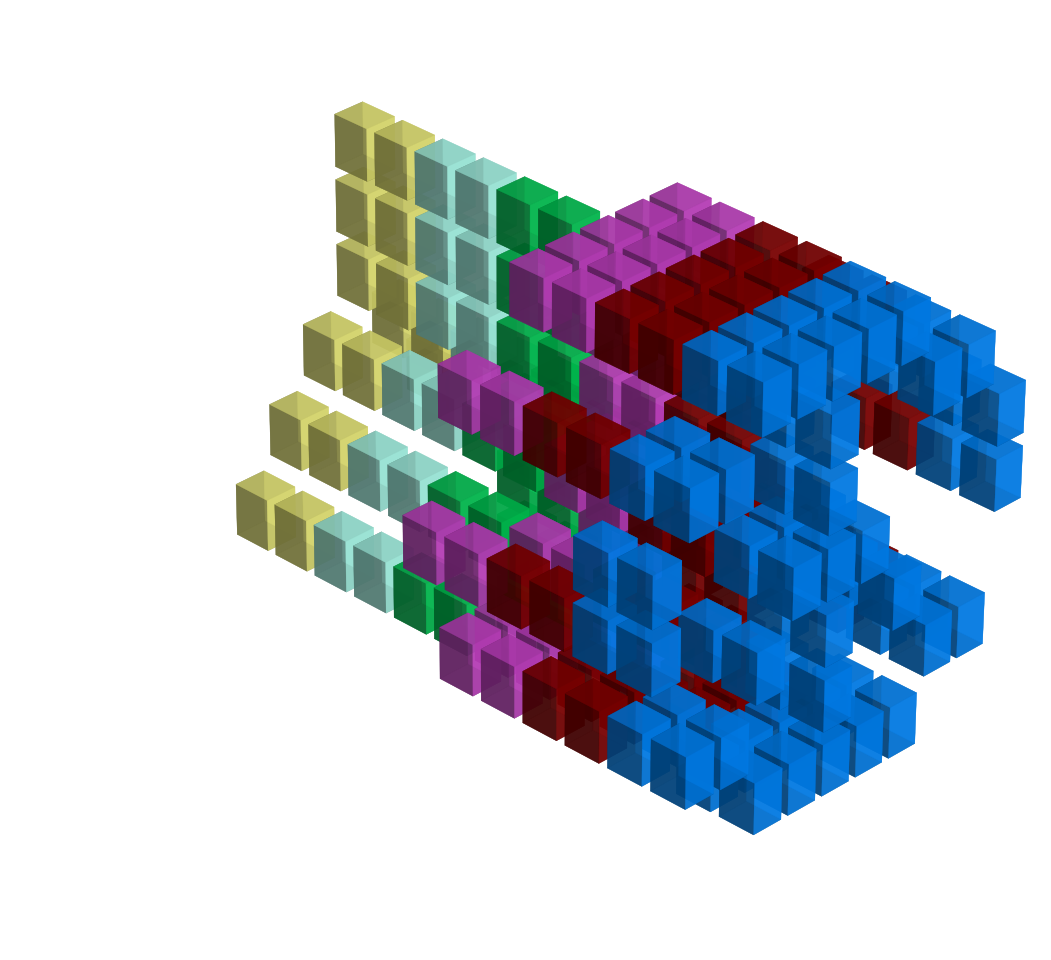
\includegraphics[width=12cm]{src/patterns/bursts/pattern3-45.png}%
    \end{adjustbox}
\caption{Evolution of the default burst at F7.}
\end{figure}
\clearpage

\rhead[]{F7 Burst}
\begin{lstlisting}[caption=Source code for the F7 Burst.,escapechar=\%]
burstGeneratorF7 = $C260
  ; currentSymmetrySetting%\index{currentSymmetrySetting}%: 'Current symmetry setting.'
  ; Possible values are 0 - 4:
  ; 'NO SYMMETRY     '
  ; 'Y-AXIS SYMMETRY '
  ; 'X-Y SYMMETRY    '
  ; 'X-AXIS SYMMETRY '
  ; 'QUAD SYMMETRY   '
  .BYTE NO_SYMMETRY
  ; smoothingDelay%\index{smoothingDelay}%: 'Because of the time taken to draw larger patterns
  ; speed increase-decrease is not linear. You can adjust the 
  ; compensating delay which often smooths out jerky patterns. 
  ; Can be used just for special FX) though. Suck it and see.'
  .BYTE $11

  ; Burst Position 1
  ; X/Y Co-ordinates: X/Y Position relative to cursor to place burst.
  .BYTE $12,$09
  ; Index to pattern in patternIndexArray%\index{patternIndexArray}%
  .BYTE CUSTOMPATTERN0

  ; Burst Position 2
  ; X/Y Co-ordinates: X/Y Position relative to cursor to place burst.
  .BYTE $12,$09
  ; Index to pattern in patternIndexArray%\index{patternIndexArray}%
  .BYTE CUSTOMPATTERN0

  ; Burst Position 3
  ; X/Y Co-ordinates: X/Y Position relative to cursor to place burst.
  .BYTE $FF,$08
  ; Index to pattern in patternIndexArray%\index{patternIndexArray}%
  .BYTE STARTWO

\end{lstlisting}

\clearpage
